% flashcards-title: The same length in two units
% flashcards-desc: One gold bar spans identical endpoints above two aligned scales. The upper scale reads zero to twenty-five centimeters and the lower scale reads zero to zero point two five meter.
\documentclass[border=5mm]{standalone}
\def\pgfsysdriver{pgfsys-dvisvgm.def}
\usepackage{tikz}
\usetikzlibrary{arrows.meta,calc,patterns.meta,positioning}
\renewcommand{\familydefault}{\sfdefault}

\definecolor{fcInk}{HTML}{1C1C1E}
\definecolor{fcMuted}{HTML}{68686D}
\definecolor{fcGuide}{HTML}{C9C9CE}
\definecolor{fcGold}{HTML}{D7A313}
\definecolor{fcGoldSoft}{HTML}{F8E8AE}

\tikzset{
  fc canvas/.style={fill=white, rounded corners=2.5mm},
  fc vector/.style={
    draw=fcGold,
    line width=1.35mm,
    line cap=round,
    -{Stealth[length=4.1mm,width=3.25mm]}
  },
  fc vector secondary/.style={
    draw=fcInk,
    line width=1.15mm,
    line cap=round,
    dash pattern=on 4.1mm off 2.6mm,
    -{Stealth[length=3.9mm,width=3.1mm]}
  },
  fc resultant/.style={
    draw=fcMuted,
    line width=1.55mm,
    line cap=round,
    -{Stealth[length=4.6mm,width=3.6mm]}
  },
  fc axis/.style={
    draw=fcInk,
    line width=.72mm,
    -{Stealth[length=3.1mm,width=2.5mm]}
  },
  fc guide/.style={
    draw=fcMuted,
    line width=.55mm,
    dash pattern=on 2.3mm off 1.8mm
  },
  fc construction/.style={draw=fcGuide, line width=.32mm},
  fc endpoint/.style={circle, fill=fcInk, inner sep=1.45mm},
  fc label/.style={font=\bfseries\large, text=fcInk},
  fc small label/.style={font=\small, text=fcMuted},
  fc caption/.style={font=\bfseries\small, text=fcMuted}
}

\begin{document}
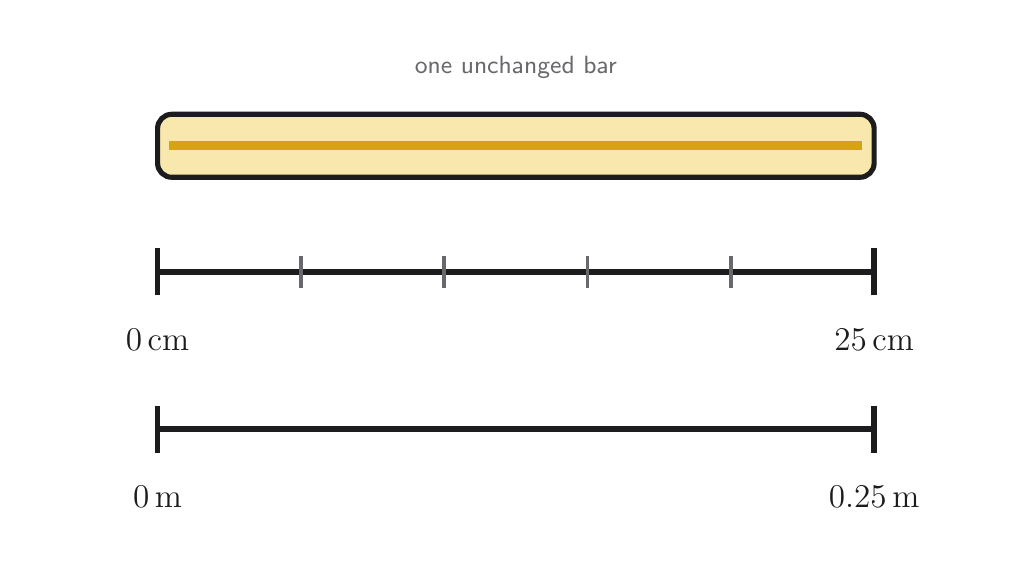
\begin{tikzpicture}[x=1cm,y=1cm]
  \path[fc canvas] (-.45,-.45) rectangle (11.95,6.25);
  \node[fc small label] at (5.75,5.75) {one unchanged bar};

  \path[draw=fcInk, fill=fcGoldSoft, line width=.65mm, rounded corners=1.8mm]
    (1.2,4.35) rectangle (10.3,5.15);
  \draw[draw=fcGold, line width=1.15mm] (1.35,4.75) -- (10.15,4.75);

  \draw[draw=fcInk, line width=.72mm] (1.2,3.15) -- (10.3,3.15);
  \foreach \x in {1.2,3.02,4.84,6.66,8.48,10.3}
    \draw[draw=fcMuted, line width=.45mm] (\x,2.95) -- (\x,3.35);
  \draw[draw=fcInk, line width=.72mm] (1.2,2.85) -- (1.2,3.45)
    (10.3,2.85) -- (10.3,3.45);
  \node[fc label, below=3mm] at (1.2,2.85) {$0\,\mathrm{cm}$};
  \node[fc label, below=3mm] at (10.3,2.85) {$25\,\mathrm{cm}$};

  \draw[draw=fcInk, line width=.72mm] (1.2,1.15) -- (10.3,1.15);
  \draw[draw=fcInk, line width=.72mm] (1.2,.85) -- (1.2,1.45)
    (10.3,.85) -- (10.3,1.45);
  \node[fc label, below=3mm] at (1.2,.85) {$0\,\mathrm{m}$};
  \node[fc label, below=3mm] at (10.3,.85) {$0.25\,\mathrm{m}$};
\end{tikzpicture}
\end{document}
